\documentclass[10pt,a4paper]{article}
\usepackage[margin=2.2cm]{geometry}
\usepackage{fontspec}
\usepackage{kotex}
\setmainfont{Apple SD Gothic Neo}
\setsansfont{Apple SD Gothic Neo}
\usepackage{amsmath,amssymb}
\usepackage{graphicx}
\usepackage{booktabs}
\usepackage{caption}
\usepackage[dvipsnames]{xcolor}
\usepackage[colorlinks=true,linkcolor=MidnightBlue,citecolor=MidnightBlue,
            urlcolor=MidnightBlue]{hyperref}
\usepackage{titlesec}
\titleformat{\section}{\large\bfseries}{\thesection}{0.6em}{}
\titleformat{\subsection}{\normalsize\bfseries}{\thesubsection}{0.5em}{}
\captionsetup{font=small,labelfont=bf}
\setlength{\parskip}{0.35em}
\setlength{\parindent}{0pt}

\usepackage{mdframed}
\newmdenv[linewidth=0.4pt,linecolor=gray!60,backgroundcolor=gray!5,
          innertopmargin=6pt,innerbottommargin=6pt,skipabove=8pt,skipbelow=8pt]{claimbox}
\newcommand{\claim}[2]{\begin{claimbox}\textbf{주장.} #1\par\smallskip
  \textcolor{gray!70}{\textbf{반증 조건.} #2}\end{claimbox}}

\title{\bfseries 부재가 측정이 됐다\\[2pt]
\large 시장팝업의 달력 --- ``걸러졌다''와 ``재지 않았다''를 가르는 법}
\author{월드모델 실험실 · 노트 $807$}
\date{2026-08-07}
\begin{document}\maketitle

\section{한 줄}

논문 $170$ 이 남긴 실마리(시장팝업의 살아 있는 열이 $3$개뿐)를 캤다. 처음 진단은
\emph{``\texttt{calaxes.SPEC} 에 시장팝업이 없다 --- 네 번째 목록 병''}이었다.
날짜는 \texttt{period\_from} 에 $249/249$ 로 준비돼 있었으니까.

\textbf{배선 게이트가 그 진단을 반쯤 무너뜨렸다.} SPEC 을 패치해도 cal 이 안
살았다 --- 둘째 문 \texttt{loop.CAL\_KEEP}$=($펀딩$\cdot$웹툰$)$ 이 있었고, 그것은
버그가 아니라 \textbf{노트 $349$ 의 측정된 절단}이다.

그런데 \texttt{git log -S} 가 셋째 사실을 줬다: \textbf{calaxes 에 시장팝업은 한
번도 없었다.} 노트 $342$ 의 도메인별 달력 지도는 cal 이 \emph{있던} 도메인만 잴
수 있었으므로, \textbf{CAL\_KEEP 의 시장팝업 제외는 측정이 아니라 부재에 의한
제외}였다. 그래서 쟀다 --- 처음으로.

\begin{center}
\begin{tabular}{lr}
\toprule
없이 & $0.1440$ \\
\textbf{진짜}(달력 $6$열) & $0.1681$ \quad (순효과 $+0.0241$) \\
위약 $6$ & $0.033{\sim}0.214$ · 평균 $0.1070$ · \textbf{뽑기 SD $0.0652$} \\
신호 몫 & $+0.0611$ \quad \textcolor{BrickRed}{문턱 $0.1303$ 미달} \\
판 변화 & $-0.0005$ \\
\bottomrule
\end{tabular}
\end{center}

\textbf{판정 (없)} --- 사전 예측($55\%$) 적중, 주 갈래 3연속.

\begin{figure}[t]\centering
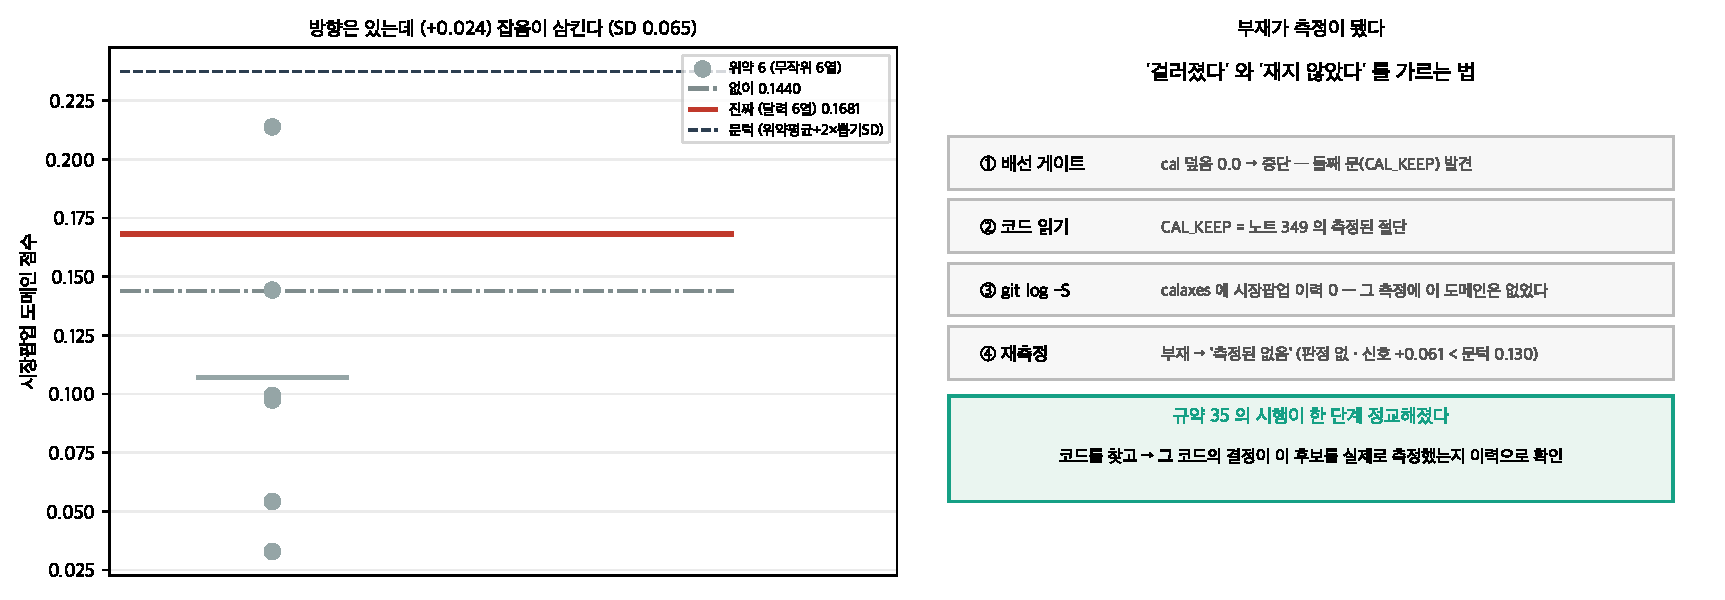
\includegraphics[width=0.92\textwidth]{figs/abs.pdf}
\caption{왼쪽: 방향은 있는데 잡음이 삼킨다. 오른쪽: 네 걸음의 판별 절차.}
\end{figure}

\section{읽을 것 둘}

\claim{\textbf{위약 평균($0.107$)이 없이($0.144$)보다 낮다} --- 무작위 $6$열은 이
도메인을 평균 $-0.037$ 깎고, 진짜 달력은 $+0.024$ 올린다. \textbf{방향은
실재한다.} 그런데 시장팝업의 열-추가 잡음(SD $0.065$)이 논문 $169$ 의 챌린저
쪽(SD $0.077$)에 이어 \textbf{판 쪽에서도 재현}됐고, 그 잡음이 어떤 $6$열
신호든 삼킨다. \textbf{이 도메인의 처방은 cal 이 아니라 trend 자료(수집) 또는
전용 열이다.}}
{$+0.024$ 가 진짜여도 지금 자로는 영영 못 가른다 --- 유보 $126$행의 $2\sigma$
($0.0233$)는 넘을 수 있지만 뽑기 SD($\times 2 = 0.130$)가 벽이다. \textbf{행이
아니라 도메인의 열-민감도가 병목인 첫 사례}로 적어 둔다.}

\claim{\textbf{규약 $35$ 의 시행이 한 단계 정교해졌다.} ``이미 걸러 둔 코드를
찾아라''의 다음 걸음: \textbf{그 코드의 결정이 이 후보를 실제로 측정했는지
이력으로 확인하라}(\texttt{git log -S}). CAL\_KEEP 은 아홉 도메인에 대해선 측정된
절단이고 시장팝업에 대해선 부재였다 --- 같은 줄의 코드가 \textbf{도메인마다 다른
인식론적 지위}를 가진다.}
{파일은 안 고쳤고 CAL\_KEEP 은 그대로다 --- 이제 그 줄은 시장팝업에 대해서도
\textbf{측정된 없음}이다. 뒤집을 조건: 시장팝업 유보가 $3$배쯤 자라거나 뽑기
잡음의 원인(축 $3$개뿐인 판에서 부스팅이 새 열에 과반응)이 따로 풀리면.}

\end{document}
